
\title{RECENT DEVELOPMENTS IN HODGE THEORY: A DISCUSSION OF TECHNIQUES AND RESULTS}
\markright{RECENT DEVELOPMENTS IN HODGE THEORY: A DISCUSSION OF TECHNIQUES AND RESULTS}

\author{By~ PHILLIP GRIFFITHS and WILFRIED SCHMID}
\markboth{PHILLIP GRIFFITHS and WILFRIED SCHMID}{RECENT DEVELOPMENTS IN HODGE THEORY: A DISCUSSION OF TECHNIQUES AND RESULTS}

\date{}
\maketitle

%\setcounter{page}{21}
\setcounter{pageoriginal}{20}


\section*{Introduction}\label{art4-sec1}
In\pageoriginale this paper, we shall review several recent developments in \textit{Hodge theory}, as applied to the study of the cohomology of algebraic varieties. In some sense, we are continuing the report \cite{art4-key21} of the first author, in which the then current work in Hodge theory was discussed without proof and a number of open problems were raised. Here we shall be concerned primarily with \textit{methods of proof}, \iec understanding in as transparent terms as possible the techniques utilized in this recent work in Hodge theory. We shall also present some results, due to the second author \cite{art4-key41}, which have just now been published, and shall bring up to date the status of the problems raised in \cite{art4-key21}.

One of the recent developments we shall discuss is Deligne's theory of \textit{mixed Hodge structures} (\cite{art4-key12}, \cite{art4-key}, \cite{art4-key14}). In this work, Deligne extends classical Hodge theory first to open, smooth varieties \cite{art4-key13}, then to complete, singular varieties \cite{art4-key14}, and finally to general varieties, also in \cite{art4-key14}. The heuristic reasoning explaining why such a theory should be possible is given in \cite{art4-key12}.

Deligne's technique is to use \textit{resolution of singularities} \cite{art4-key29}, in order to be able in each case to write the cohomology of the variety in question as being derived from the cohomology of K\"ahler manifolds by homological algebra. Typically this process gives the cohomology of the variety as the abutment of a spectral sequence whose $E_1$ or $E_2$ term is the cohomology of a smooth projective variety. Thus the $E_1$ or $E_2$ term has a \textit{Hodge structure}, and in order for this structure to survive as a Hodge structure on $E_\infty$, inducing the desired mixed Hodge structure on the cohomology of the variety, it is necessary that the spectral sequence degenerates. Following a discussion of the formalism of Hodge structures and mixed Hodge structures in \S 1, we have in \S 2 (a), \S 4, and \S 5 (d)  presented several typical degeneration arguments in as direct a manner as we could.

In \S \ref{art4-sec4} we construct the mixed Hodge structure on the cohomology of the simplest singular complete varieties, namely those having only \textit{normal crossings as singularities}. Here the main reason for the various degeneration theorems can be clearly isolated. The result in \S \ref{art4-sec4} stops far short of proving the existence of a mixed Hodge structure on the cohomology of a general singular variety \cite{art4-key14}. However, it is the method by which one most frequently \textit{calculates} this mixed Hodge structure (cf. \cite{art4-key10}, for instance), once it is known to exits.

In \S \ref{art4-sec5}, we have reproved the main result in the open case \cite{art4-key13} from a more analytic and less homological point of view. Our main idea is, instead of using the customary de Rham complex of $C^\infty$ forms on a compact K\"ahler manifold, to utilize a larger complex containing $L^1$-forms with certain precise types of singularities, and where the \textit{Gysin map} can be given on the form level preserving the Hodge filtration. This complex is discussed in \S\ref{art4-sec2}(b), where it is pointed out that the introduction of singular forms is necessary in order to have such a Gysin map on the form level. Operating inside this complex allows us to see clearly the differentials in the relevant spectral sequence in the open case, and to conclude the degeneracy result from the principle of two types (\S\S\ref{art4-sec5}(d), (e)).

Section 6 is devoted to some applications of Deligne's theory. First in \S \ref{art4-sec6}(a), we give his ``theorem on the fixed part'', which is the main tool in Deligne's study of the moduli of Hodge structures. Then, in \S\ref{art4-sec6}(b), we give a direct proof of an interesting result from \ref{art4-13}, concerning meromorphic differential forms on algebraic verieties; and finally we discuss an application of mixed Hodge structures to \textit{intermediate Jacobians} in \S \ref{art4-sec6}(c).

The second technique which we shall explore in some depth is the use of \textit{hyperbolic complex analysis}, as it applies to variation of Hodge structure. Hyperbolic complex analysis is the study of the influence of \textit{negative curvature} on holomorphic mappings. The classifying spaces for variation of Hodge structure are negatively curved, relative to the holomorphic maps which might arise in algebraic geometry (\cf. \cite{art4-key11}, \cite{art4-key25}, and \S \ref{art4-sec3}(a), (b)), and so it is natural to apply the general philosophy in this case.

Following a discussion of the basic \textit{Ahlfors lemma} and its variants in \S \ref{art4-sec7}(a), we have given Borel's proof of the quasi-unipotence of the \textit{Picard-Lefschetz transformation} in \ref{art4-sec7}(b); this should illustrate in a simple fashion the power of the method.

Perhaps the most penetrating use of the philosophy of hyperbolic complex analysis occurs in the \textit{Nevanlinna theory} \cite{art4-key24}, which affords a general mechanism for analyzing the singularities of a holomorphic mapping. Following a preliminary result from Nevanlinna theory in \S \ref{art4-sec8}(a), we have used this technique to give rather simple, geometric proofs of \textit{Borel's extension theorem} \cite{art4-sec5} in \S \ref{art4-sec8}(b), and of the \textit{Riemann extension theorem for variation of Hodge structure} \cite{art4-key19} in \S \ref{art4-sec8}(c).

A final recent development we shall discuss is the work by the second author \cite{art4-key41} and joint work by him and Clemens \cite{art4-key10}, concerning the asymptotic behavior of the Hodge structures on the cohomology groups of an algebraic variety as it acquires singularities. In \S \ref{art4-sec9}(a), we have used the theorem on \textit{regular singular points} (\S \ref{art4-sec3} (c)), together with the Ahlfors lemma, to give an alternate proof of the first theorem from \cite{art4-sec41}. This result, the \textit{nilpotent} orbit theorem, reduces the case of a general degeneration of Hodge structure to the study of a special king a \textit{nilpotent orbit} in a classifying space for variation of Hodge structure. It seems possible to use Nevanlinna theory in place of the theorem on regular singular points to prove the same result, but we have not purshed this here.

The second main theorem from \cite{art4-key41}, the $SL_2$-\textit{orbit theorem}, gives a detailed and somewhat technical description of the nilpotent orbits which can come up when a one-parameter family of Hodge structures degenerates. The proof depends heavily on Lie theory. In \S \ref{art4-sec9}(b), besides stating the theorem, we describe the observations which originally led to the proof, as well as to the statement, of the theorem.

Some applications of these two theorems will be mentioned in \S\ref{art4-sec10}; we also summarize joint results of Clements and the second author about the topology of a degenerating family of projective manifolds, which again are partly based on the two theorems.

We conclude with an appendix, reviewing the current status of the problems and conjectures contained in the report \cite{art4-sec21} of the first author.

\section{Basic definitions}\label{art4-sec1}
(a)~ \textit{Hodge structures.} Let $H_{\bR}$ be a finite dimensional real vector space, containing a lattice $H_{\bZ}$, and let $H=H_{\bR} \otimes_{\bR} \bC$ be its complexification.

\begin{definition}\label{art4-def1.1}
`A Hodge structure of weight $m$' on $H$ consists of a direct sum decomposition
$$
H = \bigotimes_{p+q=m} H^{p,q}, \text{ with } H^{q,p} = \bar{H}^{p,q}
$$
\end{definition}

(Barring denotes complex conjugation.)

\begin{remark*}
The prototypical example is the decomposition according to Hodge type of the $m$-th complex cohomology group of a compact K\"ahler manifold. In this case, $m$, $p$, $q \;\geqslant 0$; however, it will be convenient to admit also negative values for $m$, $p$, and $q$. For example, the \textit{Hodge structure of Tate} $T$(1) is defined by
$$
H_{\bZ} =\bZ, \; H_{\bR} = \bR, \; H = \bC, \; m= -2, \text{ and } H = H^{-1,-1}.
$$

For any two Hodge structures $H, H'$, both of weight $m$, the direct sum $H\oplus H'$ carries an obvious Hodge structure, also of weight $m$. Similarly, if $H$ and $H'$ have possibly different weight $m$ and $m'$,
$$
H\otimes H', \; \Hom (H, H'), \Lambda^p H, \; H^\ast
$$
inherit Hodge structures of weight $m+ m'$, $m'-m$, $pm$, and $-m$, respectively: $\lambda \in \Hom(H, H')$ has Hodge type $(p,q)$ if $\lambda(H^{r,s}) \subset (H')^{p+r, \; q+s}$ for all $r, s$; in particular, this definition applies to $H^\ast = \Hom (H, \bC)$, with $\bC$ carrying the trivial Hodge structure of weight $0; H \otimes H'$ can be identified with $\Hom (H^\ast, H')$, and $\otimes^pH$ induces a Hodge structure on its subspace $\Lambda^p H$.
 \end{remark*}

\begin{definition}\label{art4-def1.2}
A linear map $\varphi: H \to H'$ between vector spaces with Hodge structures will be called a morphism (of Hodge structures) if it is defined over $\bQ$, relative to the lattices $H_{\bZ}$, $H'_{\bZ}$, and if $\varphi (H^{p,q}) \subset (H')^{p,q}$, for all $p,q$. More generally, $\varphi$ is a morphism of type $(r,r)$ if again it is defined over $\bQ$, and if it has type ($r, r$) when viewed as an element of $\Hom(H, H')$.
\end{definition}

As a trivial, but nevertheless important, observation we note that morphism of type $(r,r)$ must vanish unless the weights $m$ and $m'$ of $H$ and $H'$ satisfy $m'=m+2r$.

To\pageoriginale each Hodge structure $H = \oplus_{p+q =m} H^{p,q}$ of weight $m$ one associates the \textit{Hodge filtration}
\setcounter{equation}{2}
\begin{equation}
H \supset \ldots \subset F^{p-1} \supset F^p \subset F^{p+1} \supset \ldots \supset 0 \text{ with } F^p = \oplus_{i \geqslant p} H^{i, m-i}.  \label{art4-eq1.3}
\end{equation}

It may be convenient to visualize the definition by means of the picture below:
\begin{figure}[H]
\centering
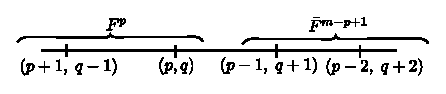
\includegraphics{art4-fig1.eps}
\end{figure}

The Hodge filtration determines the Hodge structure completely, since
\begin{equation}
H^{p,q} = F^p \cap \bar{F}^q \label{art4-eq1.4}
\end{equation}

Conversely, a descending filtration $\{F^p\}$ of $H$ arises as the Hodge filtration of some Hodge structure of weight $m$ if and only if
\begin{equation}
F^p \oplus \bar{F}^{m-p+1} \xrightarrow{\approx} H, \;\; \text{ for all } p.
\label{art4-eq1.5}
\end{equation}

Thus one has a 1:1 correspondence between Hodge structures and Hodge filtrations, \iec filtrations satisfying \eqref{art4-eq1.5}.

In terms of this latter description, a linear map $\varphi: H \to H'$, which shall be defined over $\bQ$, becomes a morphism of type $(r, r)$ exactly when it preserves the Hodge filtration, with a shift by $r$; in other words, when 
\begin{equation}
\varphi (F^p) \subset F'^{p+r}, \;\text{ for all }p. \label{art4-eq1.6}
\end{equation}

Now let $\varphi$ be a morphism of type $(r, r)$, $v$ a vector in $F'^{p+r} \cap \Iim \varphi$. By decomposing a vector in the inverse image of $v$ according to Hodge type, one finds that $v$ lies in the image of $F^p$. Thus:

a morphism of Hodge structures of type $(r,r)$ preserves the Hodge filtrations strictly, with a shift by $r$, in the sense that 
\begin{equation}
\varphi(F^p) = F'^{p+r} \cap \Iim \varphi, \text{ for all } p. 
\label{art4-eq1.7}
\end{equation}

We consider a Hodge structure $H = \oplus_{p+q = m} H^{p,q}$ and a bilinear form $Q$ on $H$, which shall be defined over $\bQ$. Also $Q$ shall be symmetric if $m$ is even, skew if $m$ is odd.

\setcounter{definition}{7}
\begin{definition}\label{art4-def1.8}
The Hodge structure is polarized by $Q$ if 
$$
\begin{matrix}
Q (H^{p,q} , H^{p', q'} =0) & \text{ unless } p = q', \; q = p',\\[2pt]
(\sqrt{-1})^{p-q} Q (v, \bar{v}) > 0 & \text{ for } v \in H^{p,q}, \; v \neq 0.
\end{matrix}
$$
\end{definition}

Apparently, the polarization form $Q$ must be nondegenerate. The Weil operator $C: H \to H$ of the Hodge structure is defined by 
\setcounter{equation}{8}
\begin{equation}
C_v = (\sqrt{-1})^{p-q} v, \text{ for } v \in H^{p,q} . \label{art4-eq1.9}
\end{equation}
In terms of the Hodge filtration and the Weil operator, the two conditions in \ref{art4-def1.8} become equivalent to 
\begin{equation}
\left.
\begin{matrix}
Q (F^p, F^{m-p+1}) = 0\\
Q (C v, \bar{v}) >0 \;\text{  for } v \neq 0.
\end{matrix}\right\}
\label{art4-eq1.10}
\end{equation}

The example we have in mind is the Hodge bilinear form on the primitive part of the cohomology of a smooth, projective variety over $\bC$, as will be discussed below.

It should be mentioned that the operations of tensor product, Hom exterior product, and duality can also be performed in the context of polarized Hodge structures. For example, if $Q$ and $Q'$ are polarization forms for Hodge structures $H$ and $H'$, then the induced bilinear form on $H \otimes H'$ polarizes the product Hodge structure.

\medskip
\noindent
(b)~ \textit{Mixed Hodge structures.} The symbols $H$, $H_{\bR}$, $H_{\bZ}$ shall have the same meaning as in the previous section.

\begin{definition}\label{art4-def1.11}
`A mixed Hodge structure' on $H$ consists of two filtrations,
$$
0 \subset \ldots \subset W_{m-1} \subset W_m \subset W_{m+1} \subset \ldots \subset H,
$$
the `weight filtration' which shall be defined over $\bQ$, and 
$$
H \supset \ldots \supset F^{p-1} \supset F^p \supset F^{p+1} \supset \ldots \supset 0,
$$
the `Hodge filtration', such that the filtration induced by the latter on $Gr_m(W_\ast) = W_m/W_{m-1}$ defines a Hodge structure of weight $m$, for each $m$ (the induced filtration on $Gr_m(W_\ast)$ is given by
$$
F^p (Gr_m (W_\ast)) = W_m \cap F^p/W_{m-1} \cap F^p).
$$
\end{definition}


\begin{remark*}
The notion\pageoriginale of a mixed Hodge structure contains that of a Hodge structure of weight $m$ as a special case; as Hodge filtration one takes the Hodge filtration in the old sense, and the weight filtration is defined by $W_m = H$, $W_{m-1} = 0$.
\end{remark*}

According to the definition of a mixed Hodge structure, only the successive quotients of the weight filtration have direct sum decompositions according to Hodge type. However, the following lemma of Deligne \cite{art4-key13} provides a more subtle global decomposition of $H$. For any pair of integers $(p,q)$, we consider the subspace
\begin{multline*}
I^{p,q} = (F^p \cap W_{p+q}) \cap (\bar{F}^q \cap W_{p+q} + \bar{F}^{q-1} \cap W_{p+q-2} +\\
 + \bar{F}^{q-2} \cap W_{p+q-3} + \ldots).
\end{multline*}
It is certainly not the case that $I^{p,q} = I^{q,p}$, but one does have the congruence $I^{p,q} \equiv I^{q,p} \mod W_{p+q-2}$, as will follow from the proof of lemma \ref{art4-lem1.12} below. This congruence $I^{p,q} \equiv \bar{I^{q,p}} \mod  W_{p+q-2}$ explains why every mixed Hodge structure with a weight filtration of length two splits over $\bR$, into a sum of two Hodge structures of pure weight. This splitting, of course, may be incompatible with the rational structure. As soon as the weight filtration has length greater than two, a ``general'' mixed Hodge structure will not split over $\bR$.

\setcounter{lemma}{11}
\begin{lemma}[\cf. Lemma 1.2.8 of \cite{art4-key13}.]\label{art4-lem1.12}
Under the projection $W_m \to Gr_m (W_\ast), \; I^{p,q}$, with $p+q=m$, maps isomorphically onto the Hodge subspace $Gr_m (W_\ast)^{p,q}$. Moreover,
$$
W_m = \oplus_{p+q\leqslant m} I^{p,q},
$$
and 
$$
F^p = \oplus_{i \geqslant p} \oplus_q I^{p,q}.
$$
\end{lemma}

\begin{proof}
In view of \eqref{art4-eq1.5}, the definition of a mixed Hodge structure amounts to the following:
\begin{align*}
& \text{given any $v \in W_n$ and integers $p,q$, with $p+q=m+1$,}\\
& \text{one can write $v = v'+\bar{v}'' + u $, such that $v' \in F^p \cap W_m$,}\\
& \text{$v'' \in F^q \cap W_m$, and $u\in W_{m-1}$; this decomposition is unique}\\
& \text{modulo $W_{m-1}$}. \tag{$\ast$}\label{art4-eq*}
\end{align*}

In order to prove the first assertion of the lemma, we fix $m$, $p$, $q$, subject to $m=p+q$, and $\alpha \in Gr_m (W_\ast)^{p,q}$. Then $\alpha$ can be represented by some\pageoriginale $v_0\in F^p \cap W_m$, and also by some $\bar{u}_0 \in \bar{F}^q \cap W_m$. Both are unique upto $W_{m-1}$, and $v_0 = \bar{u}_0 + w_0$, for some $w_0 \in W_{m-1}$. By induction on $k$, starting with $k=0$, we shall find vectors
\begin{gather*}
v_k \in F^p \cap W_m, \qquad w_k \in W_{m-1-k}\\
u_k \in F^q \cap W_m + F^{q-1} \cap W_{m-2} + F^{q-2} \cap W_{m-3} + \ldots + F^{q+1-k} \cap W_{m-k}
\end{gather*}
which will be unique up to $W_{m-k}$, such that $v_k$ represents $\alpha$, and $v_k = \bar{u}_k + w_k$. For $k=0$, this has been done $(F^{q+1} \subset F^q !)$.  If $v_k$, $u_k$, $w_k$ have been picked, we apply \eqref{art4-eq*} to $w_k$: we write $w_k = w'_k + \bar{w}''_k + w_{k+1}$, with $w'_k \in F^p \cap W_{m-1-k}$, $w_k \in F^{p-k} \cap W_{m-1-k}$, $w_{k+1} \in W_{m-2-k}$, uniquely modulo $W_{m-2-k}$. The vectors $w_{k+1}, \; v_{k+1} = v_k - w'_k$, $u_{k+1} =  u_k + w''_k$ then have the desired properties. For large enough $k$, $W_{m-1-k} = 0$; hence $\alpha$ has a unique representative in $I^{p,q}$. We may deduce that
$$
W_m = W_{m-1} \oplus (\oplus_{p+q=m} I^{p,q}),
$$
and thus $W_m = \oplus_{p+q\leqslant m} I^{p,q}$. As for the last statement of the lemma, the sum of the $I^{p,q}$ is now known to be direct. Also, one containment is obvious. We consider some $v \in F^p$, and we let $m$ be the least integer for which $v \in W_m$. The image of $v$ in $Gr_m (W_\ast)$ has Hodge components of type $(i, m-i)$, with $i \geqslant p$, because $v \in F^p \cap W_m$. Subtraction off components in the spaces $I^{i,m-i}$, with $i \geqslant p$, we can push $v$ into $W_{m-1}$. Continuing with descending induction on $m$, we find that $v \in \oplus_{i \geqslant p} \oplus \oplus_q I^{i,q}$, as was to be shown.
 
A \textit{morphism} between two mixed Hodge structures $\{H, W_m, F^p\}$,\break $\{H', W'_m, F'^p\}$ is a rationally defined linear $\map \varphi; H \to H'$, such that $\varphi(W_m) \subset W'_m$ and $\varphi (F^p) \subset F'^p$. More generally, a rationally defined linear $map \varphi : H \to H'$ will be called a morphism of mixed Hodge structures of type $(r,r)$ if $\varphi (W_m) \subset W'_{m+2r}$, $\varphi (F^p) \subset F'^{p+r}$, for all $p$ and $m$. In this case, the induced mapping
$$
\varphi: Gr_m (W_\ast) \to Gr_{m+2r} (W'_\ast)
$$
becomes a morphism of type $(r,r)$ relative to the two Hodge structures of weights $m$ and $m+ 2r$, respectively.
\end{proof}

\setcounter{lemma}{12}
\begin{lemma}\label{art4-lem1.13}
A morphism\pageoriginale of type $(r,r)$ between mixed Hodge structures is strict with respect to both the weight and Hodge filtrations, with the appropriate shift in indices. More precisely, $\varphi (W_m) = W'_{m+2r} \cap \Iim \varphi, \; \varphi (F^p) = F'^{p+r} \cap \Iim \varphi$.
\end{lemma}

\begin{proof}
The definition of the subspaces $I^{p,q}$ immediately gives the containments $\varphi(I^{p,q}) \subset I'^{p+r, q+r}$. Now let $v \in W'_{m+2r} \cap \Iim \varphi$, so that $v = \varphi (u)$ for some $u \in H$. According to \ref{art4-lem1.12},
$$
u = \sum_{p,q} u^{p,q}, \text{ with } u^{p,q} \in I^{p,q}.
$$
Then $\varphi (u^{p,q}) \in I'^{p+r , q+r}$, and $v =\sum_{p,q} \varphi (u^{p,q}) =in W'_{m+2r}$. Again appealing to \ref{art4-lem1.12}, we deduce that $\varphi(u^{p,q}) =0$, unless $p+q \leqslant m$. Hence
$$
v = \varphi \left(\sum_{p+q \leq m} u^{p,q} \right) \in \varphi (W_m).
$$

The case of the Hodge filtration is treated similarly.
\end{proof}

\begin{lemma}\label{art4-lem1.14}
Let $\varphi: H \to H'$ be a morphism of mixed Hodge structures of type $(r,r)$. Then the induced Hodge and weight filtrations put mixed Hodge structure both on the kernel and the cokernel.
\end{lemma}

\begin{proof}
As for the kernel, given $v \in \ker \varphi \cap W_m$ and any integer $p$, we must exhibit vectors
$$
v'\in \ker \varphi \cap W_m \cap F^p, \; v'' \in \ker \varphi \cap W_m \cap F^{m-p+1}, \; w \in \ker \varphi \cap W_{m-1},
$$
such that $v = v' + \bar{v}''+u$, and these must be uniquely determined modulo $\ker \varphi \cap W_{m-1}$. The uniqueness already follows from the corresponding statement about $H$. Also, there do exist $u'\in W_m \cap F^p$, $u'' \in W_m \cap F^{n-p+1}$, such that $v \equiv u' + \bar{u}'' \mod W_{m-1}$. Since $\varphi(v) = 0$, we conclude that $\varphi (u')$, $\varphi (u'') \in W'_{m+2r-1}$. By appealing to \ref{art4-lem1.12} and decomposing $u'$ into its components in the subspaces $I^{s,t} \subset H$, we can find $u'_1 \in W_{m-1} \cap F^p$, so that  $\varphi(u') = \varphi(u'_1)$. Similarly, $\varphi (u'') = \varphi (u''_1)$ for some $u''_1 \in W_{m-1} \cap F^{m-p+1}$. The vectors $v'= u'-u'_1$, $v''=u'' - u''_1$, $w = v - v'-\bar{v}''$ have the desired properties. In order to prove the assertion about the cokernel, one only has to check one nontrivial fact: if $u \in W'_m \cap F'^p$, $v \in W'_m \cap F'^{m-p+1}$, and if $u + \bar{v} \in w'_{m-1} +\Iim \varphi$, then $u, v\in W'_{m-1} + \Iim \varphi$. Using \ref{art4-lem1.12}, this can be done, in a manner similar to the argument above. Details are left to the reader.
\end{proof}

\setcounter{coro}{14}
\begin{coro}\label{art4-coro1.15}
Let $(H^\ast, d)$ be a finite dimensional complex with a mixed Hodge structure, and such that the differential $d$ is a morphism of mixed Hodge structures of type $(r,r)$, for some $r$. Then in induced filtrations on the cohomology determine a mixed Hodge structure.
\end{coro}

As a final remark, whose verification is left to the reader, we want to add the 

\setcounter{observation}{15}
\begin{observation}\label{art4-obser1.16}
Let $0 \to H' \to H \to H'' \to 0$ be an exact sequence of vector spaces. If two filtrations $\{W_l\}$ and $\{F^p\}$ for $H$ induce mixed Hodge structures on both $H'$ and $H''$, then they determine a mixed Hodge structure on $H$ itself.
\end{observation}

\section{Classical Hodge theory}\label{art4-sec2}
(a)~ \textit{The cohomology of a K\"ahler manifold}. Let $V$ be a compact, complex manifold of dimension $n$, and $A^\ast (V)$ the de Rham complex of $C^\infty$ forms on $v$. The decomposition into type
$$
A^\ast (V) = \oplus_{p,q} A^{p,q} (V)
$$
reflects the complex structure on $V$, and \textit{via} de Rham's theorem has implications in the cohomology $H^\ast (V, \bC)$. However, not very much is known about this unless $V$ is K\"ahler, or at least nearly K\"ahler. In this case, there are two main sources for the many profound implications which the complex structure plus the K\"ahler metric have in the coholomogy, and we shall briefly discuss these.

Suppose that $ds^2_V = \Sigma_{i,j} g_{ij} dz_i dz_j$ is a K\"ahler metric with fundamental (1,1)-form $\omega = \dfrac{\sqrt{-1}}{2} \Sigma_{i,j} g_{ij} dz_i \wedge d\bar{z}_j$. The operators 
\begin{align*}
& L: A^k (V) \to A^{k+2} (V)\\ 
& \wedge : A^k (V) \to A^{k-2} (V)
\end{align*} 
are defined by $L (\varphi) = \omega \wedge \varphi$ and $\Lambda =$  adjoint of $L = \pm \ast L\ast$, where $\ast : A^k (V) \to A^{2n-k} (V)$ is the duality or ``star'' operator. 

Letting 
$$
P: A^k (V) \to A^k (V)
$$
be given\pageoriginale  by $P(\varphi) = (k-n)\; \varphi$, the commutation relations
\setcounter{equation}{0}
\begin{equation}
\left.
\begin{matrix}
[L, \Lambda]  = P\\
[P, L]  = 2L\\
[P, \Lambda]  = - 2 \Lambda 
\end{matrix}
\right] \label{art4-eq2.1}
\end{equation}
exactly say that we have a Lie algebra homomorphism
$$
\rho: \fs\fl(2) \to \End (A^\ast (V)),
$$
given by 
\begin{align*}
\rho (E_+) & = L \\
\rho(E_-) & = \Lambda\\
\rho (H) & = P,
\end{align*}
where $E_+ = \left(\begin{smallmatrix}
0 & 1\\
0 & 0
\end{smallmatrix} \right)$, $E_- = \left(\begin{smallmatrix}
0 & 0\\
1 & 0
\end{smallmatrix} \right)$, and $H = \left(\begin{smallmatrix}
1 & 0\\
0 & -1
\end{smallmatrix} \right)$ are the usual basis elements for $\fs \fl$ (2). The first main source for the structure on $H^\ast(V)$ arises from the commutation relation
\begin{equation}
[\rho, \Delta] = 0 \label{art4-eq2.2}
\end{equation}
where $\Delta = dd^\ast + d^\ast d$ is the Laplacian associated to $ds^2_v$.\footnote{Here we are adopting the viewpoint of Chern \cite{art4-key7} (see also \cite{art4-key46}), where the proofs of our statements can be found. Alternate sources are \cite{art4-key45} or \cite{art-4key47}.} Letting $\sH^\ast(V) =\{\varphi \in A^{\ast} (V) : \Delta \varphi = 0\}$ be the \textit{harmonic forms} the \textit{Hodge theorem} \cite{art4-key44}.
$$
\sH^\ast (V) \xrightarrow{\approx} H^\ast_{DR} (V)
$$
together with \eqref{art4-eq2.2} tells us that $\rho$ induces a representation
\begin{equation}
\rho_\ast : \fs\fl (2) \to \End (H^\ast (V)) \label{art4-eq2.4}
\end{equation}
on the cohomology level. Applying the standard facts about representations of $\fs \fl$ to $\rho_\ast$, one obtains first the so-called \textit{Hard Lefschetz theorem}
\begin{equation}
L^k : H^{n-k} (V) \xrightarrow{\approx} H^{n+k} (V), \label{art4-eq2.4}
\end{equation}
and secondly the \textit{Lefschetz decomposition}
\begin{equation}
H^l (V) = \oplus_{0 \leqslant k \leqslant [l/2]} L^k p^{l-2k} (V), \label{art4-eq2.5}
\end{equation}\pageoriginale
where 
\begin{equation}
p^{n-k} (V) = \ker\{H^{n-k} (V) \xrightarrow{L^{k+1}} H^{n+k+2} (V)\} \label{art4-eq2.6}
\end{equation}
is the \textit{primitive part} of $(n-k)$th cohomology group.

We shall briefly discuss an application of \eqref{art4-eq2.4} and \eqref{art4-eq2.5} to prove degeneration of a spectral sequence; the argument it due to Blanchard and Deligne.

Let $X$ be a K\"{a}hler manifold (possibly non-compact), $S$ a complex manifold, and 
$$
f: X \to S
$$
a smooth, proper holomorphic mapping.\footnote{$f: X \to S$ is a differential fibre bundle whose fibres are compact K\"{a}hler manifolds; \cf. \S \ref{art4-sec3} for further discussion.} The \textit{Theorem of Leray} \cite{art4-key17} gives a spectral sequence $\{E_r\}$ with 
\begin{gather*}
E^{p,q}_2 = H^p (S, R^q_{f_\ast} (\bC))\\
E_{\infty} \Rightarrow H^\ast (X)
\end{gather*}
where the \textit{direct image sheaf} $R^\ast_{f_\ast} (\bC)$ comes from the presheaf
$$
U \to H^\ast (f^{-1} (U), \bC).
$$
The theorem asserts that $E_2 = E_\infty$.

To prove this, we remark that the K\"{a}hler metric on $X$ induces operators $L$, $\Lambda$ on the direct image sheaves $R^\ast_{f_\ast} (\bC)$ which commute with the differentials in the spectral sequence. In particular, the hard Lefschetz Theorem \eqref{art4-eq2.4} and Lefschetz decomposition \eqref(art4-eq2.5) become
\begin{gather*}
L^k : R^{n-k}_{f_\ast} (\bC) \xrightarrow{\approx} R^{n+l}_{f_\ast} (\bC)\\
R^l_{f_{\ast}} (\bC) = \oplus_k L^k P^{l-2k}_{f_\ast} (\bC),
\end{gather*}
where $P^{l-2k}_{f_\ast} = \ker \{L^{k+1}: R^{n-k}_{f_\ast} (\bC) \to R^{n+k+2}_{f_\ast}\}$. We shall check that $d_2 =0$, the proof that the higher $d_r=0$ being the same. Using the Lefschetz decomposition, it will suffice to show that $d_z =0$ on $P^{n-k}_{f_\ast} (\bC)$. Now in the diagram
$$
\xymatrix{
H^p (S, P^{n-k}_{f_\ast} (\bC)) \ar[d]^{d_2} \ar[r]^{L^{k+1}} & H^p (S, R^{n+k+2}_{f_\ast} (\bC)) \ar[d]^{d_2}\\
H^{p+2} (S, R^{n-k-1}_{f_\ast} (\bC))  \ar@{^{(}->}[r]^{L^{k+1}} & H^{p+2} (S, R^{n+k+1}_{f_\ast} (\bC)),
}
$$
the bottom row is injective by Hard Lefschetz and the top row is zero by the definition of primitivity. Thus $d_2 =0$. 

The second main source for the structure on $H^\ast(V)$ is the relation
\footnotetext[3]{This identity is \textit{equivalent} to the metric being K\"{a}hlertian}
\begin{equation}
\Delta_d = 2 \Delta_{\bar{\partial}}\footnotemark[3]{} \label{art4-eq2.7}
\end{equation}
between the Laplacians for $d$ and $\bar{\partial}$. It follows from \eqref{art4-eq2.7} that 
\begin{equation}
[\Delta, \pi_{p,q}] =0 \label{art4-eq2.8}
\end{equation}
where $\pi_{p,q} : A^\ast(V) \to A^{p,q} (V)$ is the projection onto the space of $(p,q)$-forms. Using \eqref{art4-eq2.8} and the isomorphism
$$
\sH^\ast (V) \simeq H^\ast (V, \bC), 
$$
we obtain the \textit{Hodge decomposition}
\begin{gather*}
H^m (V, \bC) = \bigoplus_{p+q=m} H^{p,q} (V), \\
H^{p,q} (V) = \bar{H^{p,q} (V)}
\end{gather*}
where $H^{p,q} (V) = \{\varphi \in A^{p,q}: d \varphi = 0\} / \{d A^\ast \cap A^{p,q}\}$.

In particular, $H^m (V, \bC)$ has a Hodge structure of weight $m$. Note that the Lefschetz decomposition is topological, whereas the Hodge decomposition reflects the complex structure (or the \textit{moduli}) of $V$.

Let us assume for the moment that the K\"{a}hler metric $ds^2_V$ is induced by a projective embedding of $V$. In this case, the K\"{a}hler operator $L$, on the cohomology level, is defined over $\bQ$. Since the fundamental form $\omega$ has Hodge type (1, 1), $L$ turns out to be a morphism of Hodge structures of type (1, 1). from this, one can deduce that the Hodge structure of $H^m (V, \bC)$ restricts to a Hodge structure on the subspace $P^m (V, \bC)$. The Hodge bilinear form
$$
Q : P^m (V, \bC) \times P^m (V, \bC) \to \bC
$$
is defined\pageoriginale by
$$
Q ([\varphi], [\psi]) = (-1)^{\frac{m(m-1)}{2}} \int\limits_v \omega^{n-m} \wedge \varphi \wedge \psi,
$$
if $\varphi$, $\psi \in A^m (V)$ represent $[\varphi]$, $[\psi] \in P^m (V)$. According to the Hodge-Riemann bilinear relations \cite{art4-key45},
$$
Q (P^m (V) \cap H^{p,q} (V), \quad P^m (V) \cap H^{p',q'} (V)) =0
$$
unless $p=q'$, $q= p'$, and 
$$
(\sqrt{-1})^{p-q} Q (c, \bar{c}) > 0 \text{ if } c \in P^m (V) \cap H^{p,q} (V), \; c \neq 0.
$$
Hence:
\begin{align}
& \text{the Hodge bilinear form $Q$ polarizes the Hodge structure}\notag \\
& \text{on the primitive part of the cohomology groups }\label{art4-eq2.9}
\end{align}
(\cf \S \ref{art4-sec1}(a)).

There are two applications of \eqref{art4-eq2.7} we want to mention. Define the \textit{Hodge filtration} on the de Rham complex by 
$$
F^pA^{\ast} (V) = \bigoplus_{i \geqslant p} A^{i,\ast} (V).
$$

\setcounter{lemma}{9}
\begin{lemma}\label{art4-lem2.10}
The exterior derivative $d$ is strict with respect to the Hodge filtration on $A^\ast(V)$. In other words, if $\varphi \in F^p A^\ast (V)$ and $\varphi = d\eta$ for some $\eta \in A^\ast (V)$, then $\eta$ can be chosen to lie in $F^p A^\ast(V)$.
\end{lemma}

\begin{proof}
Write $\varphi = \varphi_p + \varphi'$ where $\varphi' \in F^{p+1} A^\ast (V)$. Then $d\varphi = 0 \Rightarrow \bar{\partial}\varphi_p = 0$, and $\varphi = d\eta \Rightarrow \varphi_p = \partial \eta' + \bar{\partial}\eta''$ for some $\eta'$, $\eta''$. Since $\Delta_\partial=\Delta_{\bar{\partial}}$ by \eqref{art4-eq2.7}, the harmonic space for $\bar{\partial}$ is orthogonal to $\partial A^\ast (V)$, as well as to $\bar{\partial} A^\ast (V)$. Thus the $\bar{\partial}$-harmonic part of $\varphi_p$ is zero, and so $\varphi_p = \bar{\partial} \psi_p$ where $\psi_p \in F^p A^\ast (V)$. Then $\varphi - d \psi \in F^{p+1} A^\ast (V)$, and we may continue inductively.

Using the general mechanism of the spectral sequence of a filtered complex, the Hodge filtration on the de Rham complex gives rise to the Hodge - de Rham sepectral squence $\{E_r\}$ with
\begin{align*}
E_1 & = H^{\ast}_{\bar{\partial}} (A^\ast (V)), \\
E_\infty & \Rightarrow H^\ast_{DR} (V).
\end{align*}
Lemma \ref{art4-lem2.10}\pageoriginale  is equivalent to the degeneration assertion
\setcounter{equation}{10}
\begin{equation}
E_1 = E_\infty, \label{art4-eq2.11}
\end{equation}
and implies the \textit{Dolbeault isomorphism}
\begin{equation}
H^{p,q} (V) \simeq H^q (V, \Omega^p) .\label{art4-eq2.12}
\end{equation}
It also implies that the filtration on $H^\ast(V, \bC)$ induced by the filtration $F^p A^\ast (V)$ on the $C^\infty$ forms is just the usual Hodge filtration.

The second application of \eqref{art4-eq2.7} which we want to mention is the following
\end{proof}

\setcounter{lemma}{12}
\begin{lemma}\label{art4-lem2.13}
If $\varphi \in A^{p,q} (V)$ is an exact form, then we have both
\begin{align*}
\varphi & = \partial \eta' \text{ for some } \eta' \in A^{p-1,q}, \text{ with } \bar{\partial} \eta' = 0; \text{ and}\\
\varphi & = \bar{\partial} \eta'' \text{ for some } \eta'' \in A^{p,q-1} \text{ with } \partial \eta'' = 0.
\end{align*} 
\end{lemma}

\begin{proof}
The $\partial$-cohomology class of $\varphi$ is zero, and thus $\varphi = \partial \eta'$ where $\eta' = \partial^\ast G_\partial \varphi$, and $G_\partial$ is the \textit{Green's operator} for $\partial (G_\partial = \Delta^{-1}_{\partial})$ on the orthogonal complement of the harmonic space \cite{art4-key44}). Now $\eta'$ has type $(p-1, q)$; and $\bar{\partial} \eta' = 0$, since $[\partial^{\ast}, \bar{\partial}]  =0=[G_\partial, \bar{\partial}]$.
\end{proof}

The use of Lemma \ref{art4-lem2.13} comes up in the \textit{principle of two types}: If $[\varphi] \in H^m(V, \bC)$ can be represented by $\varphi' \in A^{p',q'} (V)$, and also by $\varphi'' \in A^{p'', q''} (V)$ with $p' \neq p''$, then $[\varphi] =0$. In practice, we may have a ``secondary'' cohomological construction which involves writing a cocycle as a coboundary, doing some manipulation, and then arriving at a cohomology class. This class may turn out to be zero, using \ref{art4-lem2.13} and the principle of two types, It is this heuristic reasoning which underlies the degeneration arguments for the various spectral sequences discussed in \S \S \ref{art4-sec4}, \ref{art4-sec5} below.

\medskip
\noindent
(b)~ \textit{Some comments about the Gysin mapping}. Let $V$ be a compact K\"{a}hler manifold, and $D \subset V$ a smooth divisor. Applying \textit{Poincar\'e duality} to the homology mapping
$$
H_p (D) \xrightarrow{i} H_p (V)
$$
induced by the inclusion $D \subset V$, one obtains the \textit{Gysin map}
\setcounter{equation}{13}
\begin{equation}
H^q (D) \xrightarrow{\gamma} H^{q+2}(V). \label{art4-eq2.14}
\end{equation}\pageoriginale
Since both the Poincar\'e duality isomorphisms and $i$ are morphisms of Hodge structures (of appropriate types), $\gamma$ is also a morphism, of type (1,1). We shall give a method for computing $\gamma$ on the form level; as it turns out, this cannot be done in the complex of $C^\infty$ forms, if one wants to preserve the Hodge filtration. The computation will be useful in \S \ref{art4-sec5}. In fact, the proof of the degeneration of the spectral sequence used in putting a mixed Hodge structure on the cohomology of an open variety will-follow from an obvious extension of our computation of $\gamma$ on the form level.

\medskip
\noindent
(i)~ \textsc{Definition fo Gysin mapping.} Let [$D$] be the holomorphic line bundle associated to $D$, $\sigma \in \Gamma (V, \cO[D])$ a holomorphic section with $(\sigma) = D$ and $|\sigma|$ the length function with respect to a fibre metric for $[D] \to V$. Define
\begin{equation}
\left.
\begin{matrix}
\eta = \frac{1}{2\pi \sqrt{-1}} \partial \log |\sigma|^2 \\[0.2cm]
\omega = \bar{\partial} \eta = \frac{\sqrt{-1}}{2\pi} \partial \bar{\partial} \log |\sigma|^2 ; 
\end{matrix}
\right\}
\label{art4-eq2.15}
\end{equation}
$\omega$ is a $C^\infty(1,1)$-form on $V$, which represents the dual cohomology class $c_1 ([D])$ (\cf \S 0 of \cite{art4-key24}). If $D$ is locally given by $f =0$, then 
$$
\eta = \frac{1}{2 \pi \sqrt{-1}}  \; \frac{df}{f} + \theta
$$
where $\theta$ is a $C^\infty (1,0)$ form.

\begin{defi*}
$A^\ast (\log \langle D \rangle)$ is the sub-complex of the de Rham complex $A^\ast (V-D)$ generated by $A^\ast (V)$ and $\eta$.\footnote[4]{$A^\ast (\log) \langle D \rangle$ is a special case of the $C^\infty$ \textit{log complex} associated to a divisor with normal crossings, which is discussed in \S \ref{art4-sec5} (a).
}
\end{defi*}

A form $\varphi \in A^\ast (\log \langle D \rangle)$  may be (non-uniquely) written as 
\begin{equation}
\varphi = \alpha \wedge \eta + \beta, \label{art4-eq2.16}
\end{equation}
where $\alpha, \; \beta \in A^\ast (V)$. The restriction $\alpha |_{D}$ is not ambiguous, however. Hence we may define $R: A^\ast (\log \langle D \rangle) \to A^{\ast-1} (D)$ by
\footnotetext[5]{$R$ is the \textit{Poincar\'e residue operator} discussed in \S \ref{art4-sec5}(b).}
\begin{equation}
R (\varphi) - \alpha |_{D}, \footnotemark[5]{} 
\label{art4-eq2.17}
\end{equation}\pageoriginale
and let $W^\ast \subset A^\ast (\log \langle D \rangle)$ be the kernel of $R$. There is an obvious inclusion
$$
A^\ast (V) {\displaystyle{\mathop{\hookrightarrow}\limits^i}} W^\ast,
$$
and we shall prove shortly the 

\setcounter{proposition}{17}
\begin{proposition}\label{art4-prop2.18}
The inclusion $i$ induces an isomorphism on $d$ and $\bar{\partial}$ cohomology.
\end{proposition}

Assuming this, the Gysin map on the form level is given as follows: For $\alpha \in A^{p,q} (D)$, Choose $\tilde{\alpha} \in A^{p,q} (V)$ with $\tilde{\alpha}|_D = \alpha$, and set
\setcounter{equation}{18}
\begin{equation}
\gamma(\alpha) = d (\tilde{\alpha} \wedge \eta) = d \tilde{\alpha} \wedge \eta \pm \tilde{\alpha} \wedge \omega. \label{art4-eq2.19}
\end{equation}
If $\alpha$ is a closed form on $D$, then $\gamma (\alpha)$ is a closed form in $W^\ast$ and defines a class
$$
\gamma (\alpha) \in H^\ast  (W^\ast) \simeq H^\ast_{DR} (V),
$$
using \eqref{art4-prop2.18}. We claim that this prescription, up to a factor of $\pm 1$, represents the Gysin map \eqref{art4-eq2.14}.

\begin{proof}
Given a closed form $\alpha$ on $D$ and a closed form $\psi$ on $V$, we must show that
$$
\int_V \gamma (\alpha) \wedge \psi = \pm \int_D \alpha \wedge \psi.
$$
Let $T$ be a solid tube of radius $\epsilon$ around $D$. By \eqref{art4-eq2.19} and Stokes theorem
$$
\int_V \gamma (\alpha) \wedge \psi = - \lim\limits_{\epsilon \to 0} \int_{\partial T_\epsilon} \tilde{\alpha} \wedge \eta \wedge \psi = \pm \int_D \alpha \wedge \psi,
$$
since $\lim\limits_{\epsilon \to 0} \dfrac{1}{2 \pi} \int^{2\pi}_0 f (\epsilon e^{i\theta}) d\theta = f (0)$ for any $C^\infty$ function $f$.
\end{proof}

\medskip
\noindent
(ii)~ \textsc{Comments.} (A) The forms in $A^\ast (\log \langle D \rangle)$ are \textit{integrable} on $V$, in the sense that
$$
|\int_V \varphi \wedge \psi| < \infty
$$
for\pageoriginale $\varphi \in A^\ast (\log \langle D \rangle)$ and any $\psi\in A^\ast (V)$, and thus they define \textit{currents} on $V$ (\cf. \S 2 in \cite{art4-key18}), Now $\eta$ satisfies the equation of currents.
$$
d \eta = \omega - \{D\}
$$
where $\{D\}$ is the current defined by integration over $D$, whereas the forms $\varphi \in W^\ast$ satisfy
$$
\begin{pmatrix}
d_\varphi \text{ in the }\\
\text{sense of currents}
\end{pmatrix} = 
\begin{pmatrix}
d_\varphi \text{ in the}\\
\text{sense of forms}
\end{pmatrix}
$$
This is basically the reason why \eqref{art4-prop2.18}, it follows from the discussion in $2 (a)$ that the spectral sequence associated to $F^p W^\ast$ degenerates at $E_1$, and that the induced filtration on $H^\ast (W^\ast) \cong H^\ast(V,\bC)$ is the usual Hodge filtration. Referring to \eqref{art4-eq2.19}, we see that
$$
F^p A^\ast (D) \xrightarrow{\gamma} F^{p+1} W^\ast,
$$
which again shows: \textit{The Gysin mapping \eqref{art4-eq2.14} is a morphism of Hodge structures of type} (1,1).

\medskip
\noindent
(C)~ Apropos the comment just made, we can see the necessity for going outside the class of $C^\infty$ forms in order to give $\gamma$ on the form level. If we think of $D$ as a $C^\infty$ manifold, then the extension $\tilde{\alpha}$ of $\alpha$ may be taken to be closed in a tubular neighborhood of $D$. Then $d (\eta \wedge \tilde{\alpha}) = \omega \wedge \tilde{\alpha} - \eta \wedge d \tilde{\alpha}$ is $C^\infty$ on $V$. However, if $\alpha$ lies in the pth level of the Hodge filtration, then in general we cannot find $\tilde{\alpha}$ which is closed near $D$ and is also in the pth level; the primary obstruction to doing this is a class in 
$$
H^\ast (D, \Omega^{p-1}_D [D])
$$
which may not be zero. The complex $W^\ast$ is probably the smallest one in which $\gamma$ is defined.

\medskip
\noindent
(iii)~ \textsc{Proof of \eqref{art4-prop2.18}}. First observe that the definition of $A^\ast (\log \langle D \rangle)$ and $W^\ast$ \textit{localize}: that is to say, there are obviously defined complexes of sheaves $\sA^\ast$, $\sA^\ast (\log \langle D \rangle)$, and $\sW^\ast$ on $V$ such that
\begin{align*}
& A^\ast (V) = \Gamma (V, \sA^\ast)\\
& A^\ast (\log \langle D \rangle) = \Gamma (V, \sA^\ast (\log \langle D \rangle))\\
& W^\ast = \Gamma (V, \sW^\ast).
\end{align*}
The usual sheaf-theoretic proof of de Rham's theorem will apply if we can prove the Poincar\'e lemma:\footnote[6]{The sheaves $\sA^\ast, \; \sA^\ast(\log \langle D \rangle)$, $\sW^\ast$ all satisfy $H^q (V_i) =0$ for $q > 0$.}
 
\setcounter{lemma}{19}
\begin{lemma}\label{art4-lem2.20}
The sheaf sequences on $V$
\begin{align*}
& 0 \;  \to  \; C \; \to \; \sW^0 \; {\displaystyle{\mathop{\rightarrow}^d}} \; \sW^1 \; {\displaystyle{\mathop{\rightarrow}^d}} \; \sW^2  \; \to  \; \ldots \\
& 0 \; \to \; \Omega^p_V \; \to \; \sW^p \; {\displaystyle{\mathop{\rightarrow}^{\bar{\partial}}}} \; \sW^{p,l} \; {\displaystyle{\mathop{\rightarrow}^{\bar{\partial}}}} \; \sW^{p,2} \; \to 
\end{align*}
are exact.
\end{lemma}

\begin{proof}
The problem is local around a point $p \in D$, where we choose holomorphic coordinates $(z, w ) = (z, w_1, \ldots , w_{n-1})$ on $V$ such that $D$ is given by $z=0$. Sections of $\sW^\ast$ may be written as  (\cf. \eqref{art4-eq2.16})
$$
\varphi = \alpha \wedge \frac{dz}{z} + \beta
$$
where $\alpha$, $\beta$ are $C^\infty$ forms, and where (\cf. \eqref{art4-eq2.17})
\begin{align*}
& \alpha|_{z=0} \equiv 0, \text{ and }\\
& \beta \text{ does not involve } dz.
\end{align*}
Suppose that $d\varphi = 0$ and $\deg \varphi > 0$. Write 
$$
\beta = \gamma \wedge d \bar{z}  + \delta 
$$
where $\delta$ involves only $dw$ and $d \bar{w}$. Then $d\varphi = 0 \Rightarrow d_w \delta = 0$ ($d_w$ = exterior derivative with respect to the $w$'s), and so $\delta = d_w \theta$ by the usual Poincar\'e lemma with $C^\infty$ dependence on parameters \cite{art4-key16}. Now
$$
\varphi - d\theta = \alpha' \wedge \frac{dz}{z} + \beta' \wedge d \bar{z}.
$$
where\pageoriginale $\beta'$ does not involve $dz$. Again, $d\varphi=0 \Rightarrow d_w \beta' =0$ and so $\beta' = d_w \theta' \equiv \psi \wedge \dfrac{dz}{z}$ (\mod exact forms). Write $\psi = \psi' \wedge d \bar{z} + \psi''$, where $\psi''$ involves only $dw$, $d\bar{w}$. Then $d_w \psi'' =0$ and $\psi'' |_{z=0} \equiv 0$. We may write $\psi' = d_w \eta$, with $\eta |_{z=0} \equiv 0$ \cite{art4-key16}, and then subtracting $d \left(\eta \wedge \dfrac{dz}{z} \right)$ gives
$$
\varphi = \tau \wedge d\bar{z} \wedge \frac{dz}{z} \quad  (\mod \text{ exact forms}).
$$
Once more $d_w \tau = 0$ and so $\tau = d_w \omega$, so that
$$
\varphi = \rho d \bar{z} \wedge \frac{dz}{z}, \;\; d_w \rho =0.
$$
Now $\rho = \rho (z, \bar{z})$, and by the $\bar{\partial}$-Poincar\'e lemma \cite{art4-key39}
$$
\rho d \bar{z} = \bar{\partial} \xi, \; \xi (0) = 0,
$$
so that subtracting $d \left(\xi \wedge \dfrac{dz}{z} \right)$ gives finally that $\varphi$ is exact.

The proof of the $\bar{\partial}$-Poincar\'e lemma in the present context is done in the same way, using \cite{art4-key39}.
\end{proof}

\begin{remark*}
The $\partial$-Poincar\'e lemma is \textit{false} in $\sW^\ast$; forms $f(\bar{z}) \dfrac{dz}{z}$, with $f (\bar{z})= \Sigma^{\infty}_{n=1} a_n \bar{z}^n$, are $\partial$-closed but not $\partial$-exact.
\end{remark*}

\section{Variation of Hodge structure.}\label{art4-sec3}
On a compact K\"ahler manifold, the Hodge decompositions of the complex cohomology groups reflect the complex structure of the manifold. Since a Hodge structure is a much simpler object than a global complex structure, by passing to the Hodge decompositions, one obtains a simplified model of the complex structure of the manifold. In some sense, this process is analogous to looking at the topology of a space in terms of its homology. The study of variation of Hodge structure was begun in \cite{art4-key18,key19}. We shall recall the constructions which are relevant for this paper. One can approach the subject from several points of view. Each has its advantages, and so we shall discuss and relate them in the three parts of this section. One more general comment: For technical reasons, which will become apparent below, it is necessary\pageoriginale to consider the \textit{polarized} Hodge structures on the primitive parts of the cohomology, rather than the Hodge structures on the full cohomology. Since the former completely determine the latter, no information is lost by doing so.

\medskip
\noindent
(a)~ \textit{The Hodge bundles.} Throughout this section, $X$ and $S$  will denote connected complex manifolds, and $\pi : X \to S$ a holmorphic proper mapping with connected fibres, which is everywhere of maximal rank. Moreover, $X$ is assumed to be embedded in some projective space, but not necessarily as a closed submanifold. Each fibre $V_s = \pi^{-1} (s)$, $s \in S$, then becomes a projective manifold. WE shall refer to this geometric situation as a \textit{family of polarized algebraic manifolds}.\footnote[7]{By the polarization of the fibres $V_s$, we mean the datum of the cohomology class of a projective embedding. Instead of assuming that the total space $X$ lies in some $\bP^N$, we only need a polarization for each fibre, which is constant with respect to $s$, in the sense that the polarizations form a global of the direct image sheaf $R^2_{\pi_\ast} (\bZ)$ on $S$.} In practice, such families usually arise as follows: let $\bar{X}$ and $\bar{S}$ be projective varieties and $\pi: \bar{X} \to \bar{S}$ a proper algebraic mapping, whose generic fibre is smooth. If we set $S$ equal to the subset of the regular set of $\bar{S}$ over which $\pi$ has smooth fibres, and $X= \pi^{-1} (S)$, we obtain a family of polarized algebraic manifolds.

Disregarding the complex structures, one may think of $\pi: X \to S$ as a $C^\infty$ bundle. For each integer $m$ between $0$ and $2n (n = \dim_{\bC} V_s)$, the direct image sheaf $R^m_{\pi_\ast}(\bC)$ is the sheaf of flat sections of a flat complex vector bundle $\bH^m \to S$. The fibre of $\bH^m$ over $s \in S$ has a natural identification with $H^m (V_s, \bC)$. According to harmonic theory with variable coefficients \cite{art4-key33}, the dimensions of the Hodge subspaces $H^{p,q} (V_s)$ with $p+q=m$, depend upper semicontinuously on $s$. Since their sum, being a topological invariant, remains constant, so does each of the summands. Again appealing to the results of \cite{art4-key33} one now finds that the Hodge subspaces $H^{p,q} (V_s)$ are the fibres of a $C^\infty$-subbundle $\bH^{p,q} \subset \bH^m$.  As a preliminary definition, which will soon be changed slightly, we set $\bF^p = \oplus_{i \geqslant p} \bH^{i, m-i}$. Let $\bT^\ast \to S$ be the holomorphic cotangent bundle, and  
$$
\nabla : \cO (\bH^m) \to \cO (\bH^m \otimes \bT^\ast),
$$
the\pageoriginale flat connection of $\bH^m$. The following result of the first author provides the starting point of the study of variation of Hodge structures.

\begin{theorem}[\cite{art4-key18}]\label{art4-thm3.1}
Each $\bF^p$ is a holomorphic subbundle of $\bH^m$. Furthermore,
$$
\nabla \cO(\bF^p) \subset \cO (\bF^{p-1} \otimes \bT^\ast).
$$
\end{theorem}

One can paraphrase the second statement roughly by saying that infinitesimally the subspaces $H^{p,q}(V_s)$ get shifted by a change in indices of at most one. When it is restated in terms of period matrices, as we shall do below, it looks like an infinitesimal period relation. For families of algebraic curves, this condition is vacuous. However, in the general case, it becomes a crucial ingredient of virtually all arguments about variation of Hodge structure.

The K\"{a}hler operator $L: H^m (F_s) \to H^{m+2} (V_s)$ is defined solely in terms of topological quantities.  It therefore extends to a flat bundle $\map L : \bH^m \to \bH^{m+2}$. Let $\bP^m$ be the kernel of $L^{n-m+1}$, acting on $\bH^m$. Then $\bP^m$ becomes a flat subbundle of $\bH^m$, whose fibres correspond to the subspaces $P^m (V_s) \subset H^m (V_s)$. It is the complexification of a flat real subbundle $\bP^m_{\bR}$, and $\bP^m_{\bR}$ in turn contains a flat lattice bundle $\bP^m_\bZ$. In terms of a local flat trivialization, $P^m(V_s) \cap H^{p,q} (V_s)$ is the intersection of a fixed vector space with a family of continuously varying subspaces. Hence the dimension depends semicontinuously on $s$. The sum of these dimensions, with $p + q = m$, equals the dimension of $P^m (V_s)$, which is constant. We may conclude that $\bP^m \cap \bH^{p,q}$ has constant fibre dimension, and is therefore a $C^\infty$-subbundle of $\bP^m$. Changing notation, we now set
$$
\bF^p = \oplus_{i \geqslant p} \bP^m \cap \bH^{i, m-i}.
$$
From \eqref{art4-thm3.1}, one immediately deduces the two analogous statements
\setcounter{equation}{1}
\begin{equation}
\left.
\begin{matrix}
F^p \text{ is  a holomorphic subbundle of $\bP^m$, and }\\
\nabla \cO (\bF^p) \subset \cO (\bF^{p-1} \otimes \bT^\ast). 
\end{matrix}\right] \label{art4-eq3.2}
\end{equation}
Finally, since the Hodge bilinear form $Q$ does not depend on the complex\pageoriginale structures of the fibres, we may view it as a flat bilinear form on the bundle $\bP^m$.

For some applications, it is convenient to consider collections of vector bundles with the various properties mentioned above, even if the situation does not arise directly from a family of algebraic manifolds. We gather the ingredients in the form of a definition. Let $S$ be a complex manifold. By a \textit{variation of Hodge structure, with base $S$ of weight $m$,} we shall mean a collection of the following data: 
\begin{itemize}
\item[(i)] a flat complex vector bundle $\bH \to S$, containing a flat, real subbundle $\bH_{\bR}$, so that $\bH$ is the complexification of $\bH_{\bR}$, together with a flat bundle of lattices $\bH_{\bZ} \subset \bH_{\bR}$;

\item[(ii)] a flat bilinear form $Q : \bH \times \bH \to \bC$, with $Q (f, e) = (-1)^m Q (e,f)$, which is rational with respect to $\bH_{\bZ}$;

\item[(iii)] a descending filtration of $\bH$ by a family of holomorphic subbundles $\bH \supset \ldots \supset \bF^{p-1} \supset F^p \supset \bF^{p+1} \supset \ldots \supset 0$, so that $\nabla \cO (\bF^p) \supset \cO (\bF^{p-1} \otimes \bT^{\ast})$; 
\end{itemize}
these data have to satisfy the conditions that at each $s \in S$, the fibres of the $\{\bF^p\}$ at $s$ define a Hodge structure of weight $m$ on the fibre of $\bH$, and this Hodge structure is to be polarized by $Q$.

The bilinear form $Q$ determines indefinite Hermitian metrics on the bundles $\{\bF^p\}$. It is thus possible to apply the methods of Hermitian differential geometry, as was done by the first author in \cite{art4-key19}. We shall take up these matters again in \S 10.

\medskip
\noindent
(b)~ \textit{Classifying spaces and the period mapping}. Not surprisingly, the bundles $\{\bF^p\}$ of a variation of Hodge structure can be realized as the pullbacks of certain universal bundles over a classifying space. This classifying space parametrizes the polarized Hodge structure on a fixed vector space. In order to recall the construction, which was given in \cite{art4-key18}, we consider a finite dimensional complex vector space $H$, with a real form $H_{\bR} \subset H$ and a lattice $H_{\bZ} \subset H_{\bR}$. We also fix an integer $m$ and a rationally defined bilinear form $Q$ on $H$, which shall be symmetric if $m$ is even, and skew if $m$ is odd. Next, we let $\{h^{p,q}\}$ be a collection of nonnegative integers, corresponding to pairs of\pageoriginale indices $(p,q)$ with $p+q=m$, such that $h^{q,p} = h^{p,q}$ and $\Sigma h^{p,q} = \dim H$. By $\check{D}$, we denote the set of decreasing filtrations
$$
H \supset \ldots \supset F^{p-1} \supset F^p \supset F^{p+1} \supset \ldots \supset 0
$$
which satisfy the two conditions 
\begin{equation}
\left.
\begin{matrix}
a)~~ \dim F^p = \sum_{i \geqslant p} h^{i, m-i},\\[0.2cm]
b)~~ Q (F^p, F^{m-p+1}) = 0.  \quad \quad 
\end{matrix}
\right\} \label{art4-eq3.3}
\end{equation}

In a natural way, $\check{D}$ lies as a subvariety in a product of Grassmann varieties. By elementary arguments in linear algebra one finds that the algebraic group
\begin{align}
G_{\bC} & = \text{ orthogonal group of } Q \notag\\
& = \{T \in Gl (H)| Q (Tu , Tv) = Q (u,v) \text{ for all } u, \;v \in H \} \label{art4-eq3.4}
\end{align}
operates transitively on $\check{D}$. In particular, $\check{D}$ cannot have any singularities; it is a projective manifold. The subset $D$ of all those points in $\check{D}$ which correspond to filtrations $\{F^p\}$ with the property
\begin{equation}
(\sqrt{-1})^{2p-m} Q (v, \bar{v}) > 0 \text{ if } v \in F^p \cap \overline{F^{m-p}} , \; v \neq 0, 
\label{art4-eq3.5}
\end{equation}
is open in the Hausdorff topology of $\check{D}$. Hence $D$ inherits the structure of a complex manifold from $D$. Any filtration $\{F^p\}$ belonging to a point $D$ automatically satisfies \eqref{art4-eq1.5}, and therefore determines a Hodge structure of weight $m$ on $H$ for which $Q$ is a polarization, and such that $\dim H^{p,q} = h^{p,q}$. We call $D$ a \textit{classifying space} for polarized Hodge structures, and $\check{D}$ its \textit{dual space}.

Almost by definition, the trivial vector bundle $\bH = D \times H$ over $\check{D}$ is filtered by decreasing family of holomorphic subbundles
$$
\bH \supset \ldots \supset \bF^{p-1} \supset \bF^p \supset \bF^{p+1} \supset \ldots \supset 0
$$
whose fibres over any point of $\check{D}$ constitute the filtration of $H$ corresponding to the point in question. Let $\nabla$ be the trivial flat connection on $\bH$, and $x$ a point of $\check{D}$. We shall say that a tangent vector $X$ at $x$ is \textit{horizontal} if
\begin{equation}
\nabla_x \cO (\bF^p)_x \subset \sO (\bF^{p-1})_x, \text{ for all } p. \label{art4-eq3.6}
\end{equation}
The\pageoriginale transitive action of $G_\bC$ on $D$ lifts to the family bundles $\{\bF^p\}$ and the tangent bundle. This action maps horizontal tangent vectors again to horizontal tangent vectors. In particular, the spaces of horizontal tangent vectors at the various points of $\check{D}$ have constant dimension, and they fit together, to form a $G_{\bC}$-invariant, holomorphic subbundle of the holomorphic tangent bundle $\bT \to \check{D}$. We shall call it the \textit{horizontal tangent subbundle}, $\bT_h$. A holomorphic mapping $f$ of a complex manifold $S$ into $\check{D}$, or into the open submanifold $D \subset D$, is said to be \textit{horizontal} if the induced mapping $f_{\ast}$ between the tangent spaces takes values in the horizontal tangent subbundle.

Let $G_\bR \subset G_\bC$ be the subgroup of real points,
\begin{equation}
G_{\bR} = \{T \in G_\bC | T H_{\bR} \subset H_{\bR}\} .\label{art4-eq3.7}
\end{equation}
The action of $G_{\bR}$ preserves $D \subset D$. By arguments in linear algebra (\cf \cite{art4-key18}), one can show that $G_{\bR}$ acts transitively on $D$. Thus $D$ has the structures of a homogeneous space, and this is the key to understanding all of the more subtle properties of $D$. In order to realize $D$ as a quotient space of $G_{\bR}$, we fix a \textit{base point}, or \textit{origin}, $0 \in D$. It corresponds to a filtration $\{F^p_0\}$ of $H$, the \textit{reference Hodge filtration}, which in turn determines the \textit{reference Hodge structure} $\{H^{p,q}_0\}$. The automorphism group $G_{\bC}$ of $\check{D}$ operates with isotropy group
\begin{equation}
B_\bC = \{T \in G_{\bC} | T F^p_0 \subset F^p_0 \text{ for all  } p\}\label{art4-eq3.8}
\end{equation}
at $o$; $B_{\bC}$ is a parabolic subgroup of $G_{\bC}$, and one has the identification $\check{D} \cong G_{\bC}/B_{\bC}$. We denote the group of real points in $B_{\bC}$ by $V$, \ie
\begin{equation}
V = B_{\bC} \cap G_{\bR}. \label{art4-eq3.9}
\end{equation}
Then $V$ is the isotropy subgroup of $G_{\bR}$ at $o$, and $D \simeq G_{\bR} /V$. Under these identifications, the inclusion $D \subset \check{D}$ corresponds to
\begin{equation}
D \simeq G_{\bR} / V = G_{\bR} / G_{\bR} \cap B_{\bC} \hookrightarrow G_{\bC} / B_{\bC} \simeq \check{D}. 
\label{art4-3.10}
\end{equation}
Let $C_0$ be the Weil operator of the reference Hodge structure, so that $C_0 v = (\sqrt{-1})^{p-q} v$ if $v \in H^{p,q}_0$. Since $V$ commutes with complex conjugation, it fixes not only the filtration $\{F^p_0\}$, but also the reference Hodge structure, and therefore also the positive definite hermitian form
$$
(u,v) = Q (C_0 u, \bar{v}), \quad u, \; v \in H.
$$
Hence:\pageoriginale
\begin{equation}
V \text{ is a compact subgroup of } G_{\bR}. \label{art4-eq3.11}
\end{equation}
As an arithmetic subgroup of $G_{\bR}$,
$$
\Gamma = G_{\bZ} = \{T \in G_{\bR} | T H_{\bZ} \subset H_{\bZ}\}
$$
is discrete in $G_{\bR}$. Coupled with \eqref{art4-eq3.11} and the identification $D \simeq G_{\bR} / V$, this shows:
\begin{equation}
\Gamma \text{ operates properly discontinuously on } D. 
\label{art4-eq3.12}
\end{equation}
In particular, the quotient $\Gamma \ D$ has the structures of a normal analytic space. If we had considered arbitrary Hodge structures, rather than polarized Hodge structure only, the analogous statements would be false.

Before coming back to the properties of the classifying space $D$, we recall the definition of period mapping. Let $(\bH, \bF^p)$ be a variation of Hodge structure, of weight $m$, with base space $S$---for example, the variation of Hodge structure corresponding to the $m$th primitive cohomology groups of the fibres of a family of polarized algebraic manifolds $\pi: X \to S$. The pullback of the flat vector bundle $\bH$ to the universal covering $\tilde{S}$ of $S$ is canonically trivial. Thus it makes sense  to talk of \textit{the} fibre $H$ of this pullback. The flat bundle $\bH  \to S$ is then associated to the principal bundle $\pi_1 (S) \to \tilde{S}$ by a representation $\varphi: \pi_1 (S) \to Gl (H)$. The flat subbundle $\bH_{\bR} \subset \bH$, the flat lattice bundle $\bH_{\bZ} \subset \bH_{\bR}$, and the flat pairing $Q : \bH \times \bH \to \bC$ correspond to, respectively, a real form $H_{\bR} \subset H$, a lattice $H_{\bZ} \subset H_{\bR}$, and a bilinear form $Q$ on $H$. All of these objects are preserved by the representation $\varphi$, so that $\varphi$ takes values in $\Gamma = G_{\bZ}$. The bundles $\bF^p \to S$ pull back to holomorphic subbundles of the trivial bundle $H \times \tilde{S}$. At each point of $\tilde{S}$, the fibres of these pullbacks determine a filtration of $H$, which corresponds to a Hodge structure of weight $m$ on $H$, with polarization $Q$. For these Hodge structures, the dimensions $h^{p,q} = \dim H^{p,q}$ are constant. We now consider the classifying space for Hodge structures $D$ which corresponds to the collection of Hodge numbers $\{h^{p,q}\}$. For each $s \in  \tilde{S}$, the Hodge structure determined by $s$ corresponds to a definite point in $D$. This gives a mapping $F: \tilde{S} \to D$.\pageoriginale As a direct consequence of the definition of the complex structure of $D$, $F$ is holomorphic. Also the condition (iii) for a variation of Hodge structure ensures that $F$ is a horizontal mapping. Next, if the points $s$, $s' \in \tilde{S}$ are related by an element $\gamma$ of the fundamental group of $S$, and if $T = \varphi(\gamma)$,\footnote[8]{For example, if the variation of Hodge structure arises from the $m$th primitive cohomology groups of the fibres of a family of polarized algebraic manifolds $\pi: X \to \Delta^\ast$ parametrized by the punctured disc $\Delta^\ast$, and if ${}_{\gamma \in \pi_1} (\Delta^\ast)$ is the canonical generator, $T = \varphi (\gamma)$  represents the action of $\gamma$ on the $m$th primitive cohomology group of a typical fibre $V_s$. This element $T$ is usually called the \textit{Picard-Lefschetz transformation}.} then the Hodge  structures corresponding to $s$ and $s'$ are related by $T$ : \ie $F(s') = T F (s)$. In particular, when $F$ is composed with the projection $D \to \Gamma / D$, the resulting mapping becomes $\pi_1 (S)$-invariant. Thus we obtain a mapping $f: S \to \Gamma/ D$, which is the \textit{period mapping} of the variation of Hodge structure. As follows from the construction,
\begin{align}
& \text{the period mapping is holomorphic, locally liftable,}\notag\\
& \text{and it has horizontal local liftings}. \label{art4-eq3.13}
\end{align}
By ``locally liftable'' we mean that $f$, restricted to any sufficiently small open set in $S$, factors through the projection $D \to \Gamma / D$.

This process, which associates to a variation of Hodge structure the period mapping, can almost be reversed. Let $f: S \to \Gamma / D$ be a mapping of the connected complex manifold $S$ into $\Gamma/ D$, with all of the properties mentioned in \eqref{art4-eq3.13}. Then there exists a holomorphic horizontal $\map F : \tilde{S} \to D$, which makes the diagram
$$
\xymatrix{
\tilde{S} \ar[d] \ar[r]^F & D \ar[d]\\
S \ar[r]^f & \Gamma / D
}
$$
commutative. Moreover, for each $\gamma \in \pi_1 (S)$, one can choose an element $T_{\gamma} \in \Gamma$, so that
$$
F (\gamma S) = T_{\gamma} F(s), \text{ for all } s \in \tilde{S}.
$$
Since $\Gamma$ does not operate fixed point-free, $T_{\gamma}$ may not be uniquely determined by $\gamma$\footnote[9]{This cannot happen if $f$ is ``sufficiently general''.}, in which case $\gamma \longmapsto T_\gamma$ need not be a representation of\pageoriginale $\pi_1 (S)$. However, if there does exits a homomorphism $\varphi : \pi_1 (S) \to \Gamma$, with $\varphi (\gamma) = T_\gamma$ for suitable choices of $T_\gamma$, then $\varphi$ will determine a flat bundle $\bH \to S$. All the other ingredients of a variation of Hodge structure can now also be reconstructed; details are left to the reader.

We briefly mention the classical situation, which has motivated the study of variation of Hodge structure. Let $\pi : X \to S$ be a family of principally polarized, $g$-dimensional abelian varieties, or of non-singular algebraic curves of genus $g$. The classifying space fot the Hodge structures on the first cohomology groups is then the Siegel upper half plane $H_g$, the discrete group $\Gamma$ is the Siegel moduler group, and the period mapping $f: S \to \Gamma / H_g$ associates to each fibre of the family the usual invariant in the quotient $\Gamma / H_g$.

The Siegel upper half plane, as is well known, has a realization as a bounded symmetric domain. The classifying space for the Hodge structures on the cohomology of algebraic $K3$ surfaces also has this property; it is a hermitian symmetric domain of type IV. In general however, $D$ may be very far from being a boundee domain. In fact, $D$ will usually not have any nonconstant holomorphic functions. On the other hand, the classifying spaces behave somewhat like bounded domains, as far as horizontal mappings into them are concerned. The important feature is the existence of a metric which is negatively curved in the horizontal directions. How this affects mappings into $D$ will be taken up in \S 7. Here we shall only give a precise statement about the metric in question, to which we can refer later.

\setcounter{proposition}{13}
\begin{proposition}\label{art4-prop3.14}
Let $D$ be a classifying space for Hodge structures. Then there exits a $G_{\bR}$-invariant hermitian metric on $D$, whose holomorphic sectional curvatures in all horizontal tangent directions are negative and uniformly bounded away from zero.
\end{proposition}

A general discussion of the manifolds which can arise as classifying spaces for Hodge structures is contained in \cite{art4-key25}. The proposition is proven in \S 9 of that paper. Deligne has given a short, self-contained proof in \cite{art4-key11}. Incidentally, in order to have results like \eqref{art4-prop3.14}, one is again forced to look at \textit{polarized} Hodge structures. 

proof\pageoriginale in \cite{key11}. Incidentally, in order to have results like \eqref{art4-prop3.14}, one is again forced to look at \textit{polarized} Hodge structures.

In some applications of the theory of variation of Hodge structure, one is confronted with technical problems of the following type: If $\bE \to \check{D}$ is a homogeneous, holomorphic vector bundle\footnote[10]{\ie a vector bundle to which the action of $G$ on $\check{D}$ lifts.}, and if the restriction of $\bE$ to $D$ carries a $G_{\bR}$-invariant metric, how does the metric behave as one approaches the boundary of $D$? In order to illustrate the kind of arguments which are made possible by the homogeneous  structure of $D$, we shall look at this question in particular; the answer will also be of use elsewhere in this paper.

Some preliminary remarks are needed. We recall the identification $\check{D} \simeq G_{\bC} / B_{\bC}$. A holomorphic representation $\tau: B_{\bC} \to Gl (E)$ associates a vector bundle $\bE$ to the principal bundle $B_{\bC} \to G_{\bC} \to D$. Its total space can be identified with $G_{\bC} \times E/ \sim$, with the equivalent relation $\sim$ defined by $(g^{b-1}, be) \sim (g,e)$ if $b \in B_{\bC}$. The action of $G_{\bC}$ on the first factor of $G_{\bC} \times E$ then induces an action on $\bE$ and turns $\bE$ into a homogeneous vector bundle. Conversely, every homogeneous vector bundle arises in this fashion. The restriction of $\bE$ to $D \simeq G_{\bR} / V$ may be thought of as the vector bundle associated to the principal bundle $V \to G_{\bR} \to D$ by the representation $\tau|_V$. Because of the compactness of $V$, one can choose a $V$-invariant inner product on the vector space $E$. When $E$ is identified with the fibre of $\bE$ over the origin, by translating the inner product via $G_{\bR}$, one obtains a $G_{\bR}$-invariant metric on $\bB \to D$. It should be pointed out that any two $G_{\bR}$-invariant metrics will be mutually bounded.

We are interested in comparing a $G_{\bR}$-invariant metric to a global Hermitian metric of $\bE$ over $\check{D}$, near the boundary of $D$. Since $\check{D}$ is compact, the choice of a global metric will not matter. However, there exist metrics with which one can calculate particularly easily, because they are derived from the homogeneous structure of $\check{D}$. We shall proceed to describe them. As before, $C_0$ shall denote the Weil operator of the reference Hodge structure. Then
\setcounter{equation}{14}
\begin{equation}
(u,v) = Q(C_0 u , \bar{v}), \quad u, v \in H,  \label{art4-eq3.15}
\end{equation}
defines\pageoriginale a positive definite inner product on $H$. Let $M \subset G_{\bC}$ be the intersection of $G_{\bC}$ with the unitary group of this inner product; it is a compact subgroup of $G_{\bC}$. One can check directly that
\begin{equation}
\dim_{\bR}  M = \dim_{\bC} G_{\bC} = \dim_{\bR} G_{\bR} . \label{art4-eq3.16}
\end{equation}
Next, we claim that 
\begin{equation}
M \cap B_{\bC} = V; \label{art4-art3.17}
\end{equation}
in fact, every $g \in M \cap B_{\bC}$ leaves both the reference Hodge filtration and the inner product \eqref{art4-eq3.15} invariant, and must therefore also keep the Hodge subspaces of the reference Hodge filtration fixed. In particular, $g$ commutes with $C_0$. Thus $g$ preserves the Hermitian form $Q(u,\bar{v})$, as well as the bilinear form $Q$. This is possible only if $g \in G_{\bR}$, so that
$$
M \cap B_{\bC} \subset G_{\bR} \cap B_{\bC} = V.
$$
The reverse containment is clear, and \eqref{art4-eq3.17} is proven. Then $M$-orbit of the origin in $\check{D}$ can now be indentified with $M/V$; because of \eqref{art4-eq3.16}, it has the same dimension as $D \simeq G_{\bR} / V$ and must be open in $D$. On the other hand, the compactness of $M$ forces the orbit to be closed. Thus
\begin{align}
& \text{$M$ operates transitively on $\check{D}$, with isotopy group $V$.} \notag\\
& \text{at the origin, so that $\check{D} \simeq M / V$.}\label{art4-eq3.18}
\end{align}
Just as a $V$-invariant inner product on $E$ gives rise to a $G_{\bR}$- invariant Hermitian metric for $\bE \to D$, such an inner product can be translated around by $M$, to give an $M$, to give an $M$-invariant Hermitian metric for $\bE$ over all of $\check{D}$.

We now consider two Hermitian metrics $h_1, h_2$ for $\bE$ of which the first is $G_{\bR}$-invariant and defined over $D$, and the second $M$-invariant and defined over  all of $\check{D}$. We also assume that the two metrics coincide on the fibre over the origin. Let $x$ be a point of $D$ and $e$ a vector in the fibre of $\bE$ over $x$. We can write $x$ as the $g$-translate of the origin, for some $g \in G_{\bR}$, and also as the $m$-translate of the origin, for some $m \in M$. Since $B_\bC$ is the isotropy subgroup of $G_{\bC}$ at the origin, $g = mb$, with $b \in B_{\bC}$. In order to compute the $H_1$-length of $e$, we may translate $e$ by $g^{-1}$ to the origin and compute the length there.\pageoriginale Similarly, the $h_2$-length of $e$ is the length of its translate by $m^{-1}$ at the origin. It follows that $h_1$ and $h_2$ at $x$ are mutually bounded by, respectively, the operator norm of $\tau(b)$ and the operator norm of $\tau (b^{-1})$, relative to the $V$-invariant inner product on $E$ which corresponds to the two metrics. The matrix entries of $\tau (b)$ and $\tau (b^{-1})$ are rational functions of those of $b$, when $b$ is viewed as an element of the matrix group $G_{\bC}$. Because of the compactness of $M$, the matrix entries of $b = m^{-1} g$ are bounded by a constant multiple of the largest matrix entry of $g$. For any $g \in G_{\bR}$, we let $||g||$ denote the operator norm of $g$ on $H$, relative to some inner product on $H$. According to what has been argued above, the metrics $h_1$ and $h_2$ on the fibre of $\bE$ over $x$ must be mutually bounded by a constant multiple of a suitable power of $||g||$. Clearly this remains correct if we replace $h_1$ by any $G_\bR$-invariant metric and $h_2$ by any global Hermitian metric for $\bE$ over all of $\check{D}$. We have proven:

\setcounter{lemma}{18}
\begin{lemma}\label{art4-lem3.19}
Let $\bE \to \check{D}$ be a homogeneous holomorphic vector bundle, $h_1$ a $G_{\bR}$-invariant metric for the restriction of $\bE$ to $D$, and $h_2$ a global Hermitian metric for $\bE$ over $\check{D}$. There exist constants $C, N$ with the following property : if $x \in D$ is the $g$-translate of the origin, with $g \in G_{\bR}$, then each of the two metrics $h_1, h_2$ at $x$ is bounded by $C ||g||^N$ times the other.
\end{lemma}

In order to make the lemma useful, one has to know how $||g||$ grows as the point $x$ approaches the boundary of $D$. For this purpose, we recall some standard facts from the theory of symmetric spaces.\footnote[11]{Helgason's book \cite{art4-key27} is a good reference.} Let $G_{\bR}$ be a semisimple matrix group, and $K \subset G_{\bR}$ a maximal compact subgroup. The quotient $G_{\bR} / K$ then carries a $G_{\bR}$-invariant, Riemannian metric $ds^2$, which is essentially unique. In the Lie algebra of $\fg_0$ of $G_{\bR}$, the subagebra $\fk_0$ corresponding to $K$ has a unique Ad $K$-invariant complement $\fp_0$. We now choose a maximal abelian subspace $\fa_0$ in $\fp_0$, and we denote the subgroup exp $\fa_0$ of $G_{\bR}$ by $A$. All elements of $A$ act semisimply, under any finite dimensional representation of $G_{\bR}$. One then has the (non-unique) decomposition
\setcounter{equation}{19}
\begin{equation}\label{art4-eq3.20}
G_{\bR} = K \; A  \; K.
\end{equation}\pageoriginale
Moreover, with respect to a suitable Euclidean metric on $\fa_0$,\footnote[12]{If the Riemannian structure $ds^2$ is the one corresponding to the Killing form, the restriction of the Killing form to $\fa_0$ will be the ``suitable Euclidean metric''.}
\begin{align}
& X \longmapsto \exp XK \text{ is a locally and globally isometric,}   \notag\\
& \text{totally geodesic embedding of $A$ in $G_{\bR}/K$.} \label{art4-eq3.21}
\end{align}

In our situation, as the ``orthogonal group'' of a nondegenerate, symmetric or skew symmetric bilinear form, $G_{\bR}$ will certainly be semisimple. Because of \eqref{art4-eq3.11}, there exists a maximal compact subgroup $K$ of $G_{\bR}$ which contains $V$. Relative to any two $G_{\bR}$ invariant metrics, the projection
\begin{equation}
D\simeq G_{\bR} / V \to G_{\bR} / K
\label{art4-eq3.22}
\end{equation}
is bounded. Let $x \in D$ be the $g$-translate of the origin, with $g \in G_{\bR}$. We write $g = k_1 a k_2, k_1, k_2 \in K$, $a \in A$. According to \eqref{art4-eq3.21} and the boundedness of the projection \eqref{art4-eq3.22}, the Euclidean norm of log $a$ is bounded by some multiple of the distance $\rho_D (x,0)$. The abelian group $A$ can be simultaneously diagonalized, because all of its elements operate semisimply. Hence the operator norm of $a$ cannot exceed some multiple of a suitable power of $\exp \rho_D (x, 0)$. Since $g = k_1 a k_2$, and since $K$ is compact, this gives the same kind of estimate also for the operator norm of $g$. Thus:

\setcounter{lemma}{22}
\begin{lemma}\label{art4-lem3.23}
There exist positive constants $B$, $M$, with the following property: if $x \in D$ is the $g$-translate of the origin, with $g \in G_{\bR}$, then
$$
||g|| \leqslant B \exp M_{\rho_D} (X,0).
$$
\end{lemma}

With this lemma, the comparison of the metrics in \eqref{art4-lem3.19} can now be rephrased in a more intrinsic manner.

\medskip
\noindent
(c)~ \textit{Period matrices.} In his book \cite{art4-key30} on harmonic integrals, Hodge phrased his results on the cohomology of K\"ahler manifolds in the language of \textit{period matrices}. For some questions, such as computations of specific examples, it is useful to be able to think in this way, and so we shall give a brief ``dictionary'', relating the preceding discussion to the language of period matrices. This description\pageoriginale of Hodge structures will be used in \S \S 8, 9 below. We conclude this section with a proof of the theorem of the regularity of the connection on the Hodge bundles.

Let us consider a polarized Hodge structure $\{H^{p,q}\}$ of weight $m$ on the vector space $H$, with polarization form $Q$. Once and for all, we assume that $H^{p.q} =0$ unless $p, q \geqslant 0$. Also to simplify the discussion, we shall limit ourselves mainly to the case when $m =2$, with only some parenthetical remarks about the general case. Under these hypotheses, the Hodge filtration has length 2:
\begin{equation}
H = F^0 \supset F^1 \supset F^2 \supset 0. \label{art4-eq3.24}
\end{equation}
For $0 \leqslant k \leqslant 2$, $F^k$ and $F^{3-k}$ are perpendicular with respect to $Q$. On the other hand, $Q$ is nondegenerate, and $F^k$ and $F^{3-k}$ have complementary dimensions, so that $F^{3-k} = F^{k \bot}$. As an immediate consequence, we see that $F^2$ already determines the remaining subspaces.\footnote[13]{In general, it suffices to know $F^k$, for $[m/2] + 1 \leqslant k \leqslant m$; if $k \leqslant [m/2]$, $F^k$ is then determined by $F^k = (F^{m-k+1})^\bot$.} We now let the polarized Hodge structure vary, keeping the polarization form $Q$ and the Hodge number $r = \dim H^{2,0} = \dim H^{0,2}$ and $s = \dim H^{1,1}$ fixed. The points of the dual space $\check{D}$ of the classifying space $D$ then correspond exactly to the subspaces
\begin{equation}
F^2 \subset H, \text{ with } \dim F^2 = r , \; Q (F^2, F^2) = 0. 
\label{art4-eq3.25}
\end{equation}
Such a subspace can be completed to a filtration  \eqref{art4-eq3.24} by setting $F^1 = F^{2\bot}$. The subspace belongs to a point of $D$ when the appropriate positivity conditions are satisfied. In our special case, they can be compressed into the single condition
\begin{equation}
- Q (v, \bar{v}) > 0 \text{ if } v \in F^2, \; v \neq 0.
\label{art4-eq3.26}
\end{equation}
Indeed, by conjugation, the condition on $H^{0,2}$ follows from \eqref{art4-eq3.26}, and the condition on $H^{1,1} = (H^{2,0} \otimes H^{0,2})^\bot$ is automatic, since $Q$ has exactly $s$ positive eigenvalues.
 
In order to represent the points of $D$ and $\check{D}$ by period matrices, we pick a basis $\{e_1,\ldots, e_{2r+s}\}$ of the lattice $H_{\bZ}$, and we denote the dual basis by $\{\lambda^1, \ldots, \lambda^{2r+s}\}$. Relative to the basis $\{e_i\}$, the bilinear form $Q$ is specified by a $(2r+s) \times (2r+s)$ matrix, which we shall also call $Q$. Given a subspace $F^2$ as in \eqref{art4-eq3.25}, we choose a basis $\{v_1, \ldots, v_r\}$, and we\pageoriginale let $\Omega$ be the $(2r+s) \times r$ matrix whose $(i,j)$-entry is $\langle \lambda^i, v_j\rangle $; this is the period matrix of the Hodge structure in question\footnote[14]{For arbitrary $m$, one obtains a collection of $[(m+1)/2]$ period matrices, corresponding to the subspaces $F^k, [m/2] +  1 \leqslant k \leqslant m$.} It clearly determines the Hodge structure completely. Every nonsingular $(2r+s) \times r$ matrix $\Omega$ which satisfies the first of the two bilinear relations
\begin{equation}
\left.
\begin{aligned}
{}^t \Omega Q \Omega & = 0\\
- {}^t \Omega Q \bar{\Omega} & > 0
\end{aligned}
\right\}\label{art4-eq3.27}
\end{equation}
corresponds to a point of $D$. If it satisfies the second relation as well, hen it is the period matrix of an actual Hodge structure. Two such matrices $\Omega$ and $\Omega'$ belong to the same point of $\check{D}$, or of $D$ exactly when $\Omega' = \Omega A$, for some invertible $r \times r$ matrix $A$. This equivalence relation reflects the freedom of choice of a basis of $F^2$. In the preceding discussion, the basis $\{e_i\}$ of $H_{\bZ}$ has been kept fixed; changing it has the effect of pre-multiplying the period matrices by the transpose of the change-of-base matrix.

The set of tall nonsingular $(2r+s) \times r$ matrices $\Omega$, modulo the equivalence relation $\Omega \sim \Omega A$, is a particular realization of the Grassmannian $Gr (r, 2r + s)$ of $r$-planes in $\bC^{2r+s}$. The first of the two bilinear relations \eqref{art4-eq3.27} exhibits $\check{D}$ as a sub-variety of this Grassmannian. By associating to each nonsingular matrix $\Omega$ the \textit{Pl\"ucker coordinates}
$$
\Omega_{i_1, \ldots ,i_r} = \det 
\begin{bmatrix}
\Omega_{i_1, 1} & \ldots & \Omega_{i_1, r}\\
\vdots & & \\
\Omega_{i_r,1} &  \ldots & \Omega_{i_r, r}
\end{bmatrix},
$$
one obtains the Pl\"ucker embedding of $Gr (r, 2r + s)$, and thereby also of its subvariety $\check{D}$, in the projective space of dimension $\begin{pmatrix}2r + s\\r\end{pmatrix}- 1$. The set of period matrices forms the total space of a holomorphic principal bundle over $\check{D}$, with structure group $Gl(r,\bC)$. The character of\pageoriginale $Gl(r,\bC)$ induces a holomorphic line bundle $\bL \to D$, whose space of sections has the Pl\"{u}cker coordinates $\Omega_{i_1, \ldots, i_r} $ as a basis.

Like any principal bundle, the bundle of period matrices has local section. Hence every holomorphic mapping $f : S \to D$ can be represented locally by a holomorphic, matrix-valued function $\Omega(s)$, $s \in S$, whose values satisfy the two bilinear relations \eqref{art4-eq3.27}. The mapping $f$ is horizontal exactly when the column vectors of $d \Omega$ correspond to one-forms with values in $F^1 = F^2 \bot$; in other words, when
\begin{equation}
{}^t \Omega (s) Q d \Omega (s) = 0,
\label{art4-eq3.28}
\end{equation}
which looks like an infinitesimal period relation.

We now consider a variation of Hodge structure with base $S$;\footnote[15]{The assumptions made at the beginning of this section still apply.} or, more concretely, the periods of holomorphic two-forms for a polarized family of algebraic manifolds $\pi: X \to S$. We fix a base point $s_0 \in S$, and we choose a basic $\{e_i\}$ of the fibre of $\bH_{\bZ}$ over $s_0$. In the geometric situation, this amounts to choosing a basis for the primitive part of $H_2 (V_{s_0}, \bZ)$. Displacing the $e_i$ horizontally, we obtain a flat frame $\{e_i(s)\}$, $s \in \tilde{S}$, for the pullback of $\bH_{\bZ}$ to the universal covering $\tilde{S}$ of $S$. If $\varphi : \pi_1 (S) \to G_{\bZ} = SO (Q, \bZ)$ is the representation corresponding to the flat bundle $\bH \to S$, one finds that 
\begin{equation}
e_i (\gamma s ) = \varphi (\gamma) e_i (s), \text{ whenever } \gamma \in \pi_1 (S), \; s \in \tilde{S}. 
\label{art4-eq3.29}
\end{equation}
It may be possible to find a holomorphic frame $\{\sigma_1, \ldots, \sigma_r\}$ of the bundle $\bF^2 \to S$, although usually only outside of a subvariety of $S$. By pairing the $\sigma_i's$ with the dual frame to $\{e_i (s)\}$, we obtain a holomorphically varying period matrix $\Omega (s)$, $s \in \tilde{S}$, which describes the period mapping.\footnote[16]{For a general $m$, this process yields a collection $\{\Omega_i (s)\}$ of $\left[\dfrac{m+1}{2}\right]$ matrix valued functions.} The transformation property \eqref{art4-eq3.29} implies 
\begin{equation}
\Omega (\gamma s) = \varphi (\gamma) \Omega (s), \text{ for } \gamma \in \pi_1 (S), \; s \in \tilde{S}.  \label{art4-eq3.30}
\end{equation}
Equivalently, we may think of $\Omega (s)$ as a \textit{multiple-valued} function on $S$.

We shall use the language of period matrices to sketch a proof of the theorem on regular singular points. Let $\pi : X \to \Delta^\ast$  be a family of polarized algebraic manifolds over the punctured disc $\Delta^\ast = \{z \in \bC | 0 < |z| < 1\}$, 

%%%%% 66






\begin{thebibliography}{99}
\bibitem{art4-key1}
\end{thebibliography}





